\documentclass[a4paper]{article}

\setlength{\textwidth}{16cm}
\usepackage[T1]{fontenc}
\usepackage[english]{babel}
\usepackage{amsmath, amsfonts}
\usepackage{graphicx}
\usepackage{alltt}
\usepackage{hyperref}
\usepackage{lmodern}
\usepackage{hyperref}
\usepackage{tikz}
\usepackage{gensymb}
\usepackage[titletoc]{appendix}
\usepackage{tabto}
\usepackage{float}
\usepackage{dashrule}
\usepackage{subfig}
\usetikzlibrary{intersections,calc}
\usepackage{pdfpages}
\usepackage{listings}
\usepackage{color}
\usepackage{caption}
\usepackage{newclude}
\usepackage{enumitem}
\usepackage{tabularx}
\usepackage[utf8]{inputenc}
\usepackage{fancyhdr}
\usepackage{geometry}
\usepackage{pdfpages}
\usepackage{numprint}
\usepackage{multirow}
\usepackage{arydshln}
\usepackage{titlesec}
\usepackage[titletoc]{appendix}
\usepackage{chngcntr}
\usepackage{cleveref}
\newcommand{\aref}[1]{\hyperref[#1]{Appendix~\ref{#1}}}
\counterwithin{table}{section}
\counterwithin{figure}{section}
\setlength\dashlinedash{0.3pt}
\setlength\dashlinegap{3pt}
\pagenumbering{arabic} 
\begin{document}
%%%%%%%%%%%%%%%%%%%%%%%%%%%%%%%%%%%%%%%%%%%%%%%%%%%%%
\titleclass{\subsubsubsection}{straight}[\section]

\newcounter{subsubsubsection}[subsubsection]

\renewcommand{\labelenumii}{\arabic{enumi}.\arabic{enumii}}
\renewcommand{\labelenumiii}{\arabic{enumi}.\arabic{enumii}.\arabic{enumiii}}
\renewcommand{\labelenumiv}{\arabic{enumi}.\arabic{enumii}.\arabic{enumiii}.\arabic{enumiv}}

\renewcommand\thesubsubsubsection{\thesubsubsection.\arabic{subsubsubsection}}
\renewcommand\theparagraph{\thesubsubsubsection.\arabic{paragraph}}
\renewcommand\thesubparagraph{\theparagraph.\arabic{subparagraph}}

\titleformat{\subsubsubsection}
  {\normalfont\normalsize\bfseries}{\thesubsubsubsection}{1em}{}
\titlespacing*{\subsubsubsection}
{0pt}{3.25ex plus 1ex minus .2ex}{1.5ex plus .2ex}

\makeatletter
\renewcommand\paragraph{\@startsection{paragraph}{5}{\z@}%
  {3.25ex \@plus1ex \@minus.2ex}%
  {-1em}%
  {\normalfont\normalsize\bfseries}}
\renewcommand\subparagraph{\@startsection{subparagraph}{6}{\parindent}
  {3.25ex \@plus1ex \@minus .2ex}%
  {-1em}%
  {\normalfont\normalsize\bfseries}}
\def\toclevel@subsubsubsection{4}
\def\toclevel@paragraph{5}
\def\toclevel@paragraph{6}
\def\l@subsubsubsection{\@dottedtocline{4}{7em}{4em}}
\def\l@paragraph{\@dottedtocline{5}{10em}{5em}}
\def\l@subparagraph{\@dottedtocline{6}{14em}{6em}}
\@addtoreset{subsubsubsection}{section}
\@addtoreset{subsubsubsection}{subsection}
\@addtoreset{paragraph}{subsubsubsection}
\makeatother

\setcounter{secnumdepth}{6}
\setcounter{tocdepth}{6}

%%%%%%%%%%%%%%%%%%%%%%%%%%%%%%%%%%%%%%%%%%%%%%%%%%%

\pagestyle{fancy}
\thispagestyle{empty}
\noindent
\textbf{Experiment 5}\hfill \\
\textbf{Date:03-06-2022}
\hfill
\title{Lab report}
\begin{center}
\vspace{15mm}
\textbf{\Huge {CPU Scheduling Algorithm}}
\end{center}
\vspace{2.5pt}

\textbf{{\Large Aim
}}\\
\vspace{1.5pt}
\par To implement the following CPU scheduling algorithms :\par a)Round Robin\par b)SJF\par c)FCFS\par d)Priority
\vspace{1.5pt
}
\section{Round Robin Scheduling}

\subsection{Aim}
To write a C program that implements Round Robin algorithm.

\subsection{Algorithm}
\begin{enumerate}
\item Start
\item Read the number of processes to pro
\item Read the arrival time and burst time of the processes
\item Read the Quantum Number to qn
\item Sort the processes in the increasing order of the arrival time
\item Initialize time=a[0].arrivaltime, remain=pro
\item For i=0 and remain!=0
\begin{enumerate}
\item If remaining burst time less than qn and greater than 0, time = time+a[i].remainingtime and print process number and time, set a[i].remainingtime=0 and flag=0
\item Else if remaining burst time is greater than 0, a[i].remainingtime =a[i].remainingtime-qn, time=time+qn, print process number and time
\item If a[i].remainingtime=0 and flag=1
\begin{enumerate}
\item Decrement remain
\item a[i].turnaroundtime = time-a[i].arrivaltime
\item a[i].waitingtime = a[i].turnaroundtime-a[i].bursttime
\item avgwt = avgwt + a[i].waitingtime
\item avgtt = avgtt + a[i].turnaroundtime
\item flag=0
\end{enumerate}
\item If i=pro-1, i=0
\item Else if a[i+1].arrivaltime less than time, increment i else i=0 
\end{enumerate}
\item Average waiting time = avgwt/pro
\item Average Turnaround time = avgtt/pro
\item Print turnaround time and waiting time of each process and average waiting time and turnaround time
\item Stop
\end{enumerate}
\subsection{Program}
\lstinputlisting{roundrobin.c}
\\
\\
\subsection{Sample Input and Output}
\begin{figure}[!h]
	\centering
	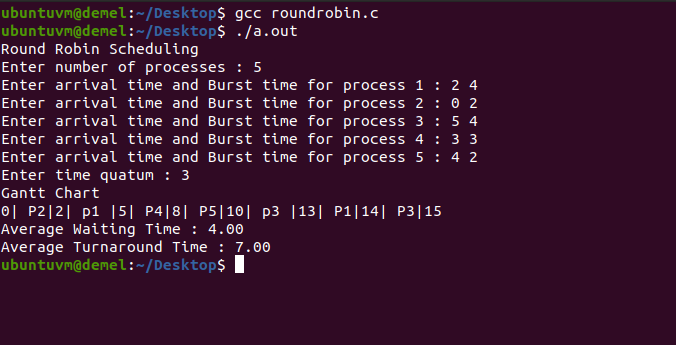
\includegraphics[width=\textwidth]{roundrobin.png}
\end{figure}

\section{First Come First Serve Scheduling}

\subsection{Aim}
To write a C program that implements FCFS algorithm.

\subsection{Algorithm}
\begin{enumerate}
\item Start
\item Read the number of processes to pro
\item Read the arrival time and burst time of the processes
\item Sort the processes in the increasing order of the arrival time
\item Initialize time=arrival time of first process
\item For i=0 until i<pro repeat the following
\begin{enumerate}
\item time = time+a[i].bursttime
\item a[i].turnaroundtime = time-a[i].arrivaltime
\item a[i].waitingtime = a[i].turnaroundtime-a[i].bursttime
\item avgwt = avgwt + a[i].waitingtime
\item avgtt = avgtt + a[i].turnaroundtime
\item Print process number and time
\item If i not equal to pro-1 and a[i+1].arrivaltime > time, time=a[i+1].arrivaltime and print time
\end{enumerate}
\item Average waiting time = avgwt/pro
\item Average Turnaround time = avgtt/pro
\item Print turnaround time and waiting time of each process and average waiting time and turnaround time
\item Stop
\end{enumerate}
\subsection{Program}
\lstinputlisting{fcfs.c}
\\
\newpage
\subsection{Sample Input and Output}
\begin{figure}[!h]
	\centering
	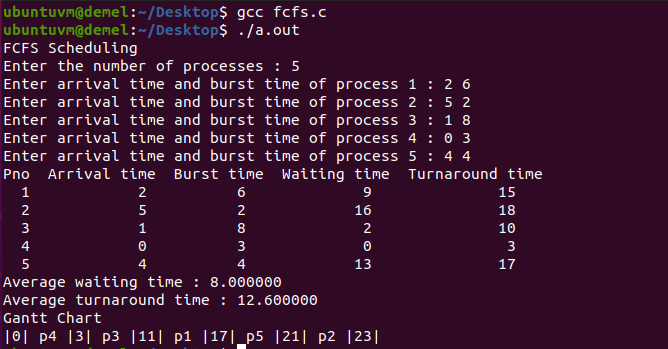
\includegraphics[width=\textwidth]{fcfs.png}
\end{figure}

\section{Shortest Job First Scheduling}

\subsection{Aim}
To write a C program that implements SJF algorithm.

\subsection{Algorithm}
\begin{enumerate}
\item Start
\item Read the number of processes to pro
\item Read the arrival time and burst time of the processes
\item Sort the processes in increasing order of burst time
\item Initialize time=arrival time of process with smallest arrival time, remain=pro
\item For i=0 until remain not equal to 0 repeat the following
\begin{enumerate}
\item Choose a process i who has smallest burst time and arrival time less than or equal to time, if not available next process with smallest arrival time
\item If i not equal to pro-1 and a[i+1].arrivaltime > time, time=a[i+1].arrivaltime and print time
\item time = time+a[i].bursttime
\item a[i].turnaroundtime = time-a[i].arrivaltime
\item a[i].waitingtime = a[i].turnaroundtime-a[i].bursttime
\item avgwt = avgwt + a[i].waitingtime
\item avgtt = avgtt + a[i].turnaroundtime
\item Print process number and time
\end{enumerate}
\item Average waiting time = avgwt/pro
\item Average Turnaround time = avgtt/pro
\item Print turnaround time and waiting time of each process and average waiting time and turnaround time
\item Stop
\end{enumerate}
\subsection{Program}
\lstinputlisting{sjf.c}
\\

\subsection{Sample Input and Output\\}
\begin{figure}[!h]
	\centering
	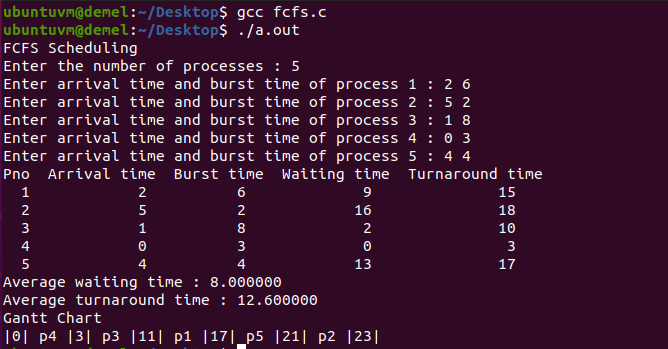
\includegraphics[width=\textwidth]{fcfs.png}
\end{figure}


\section{Priority Scheduling}

\subsection{Aim}
To write a C program that implements Priority scheduling algorithm.

\subsection{Algorithm}
\begin{enumerate}
\item Start
\item Read the number of processes to pro
\item Read the priority, arrival time and burst time of the processes
\item Sort the processes in increasing order of priority
\item Initialize time=arrival time of process with smallest arrival time, remain=pro
\item For i=0 until remain not equal to 0 repeat the following
\begin{enumerate}
\item Choose a process i who has smallest burst time and arrival time less than or equal to time, if not available next process with smallest arrival time
\item If i not equal to pro-1 and a[i+1].arrivaltime > time, time=a[i+1].arrivaltime and print time
\item time = time+a[i].bursttime
\item a[i].turnaroundtime = time-a[i].arrivaltime
\item a[i].waitingtime = a[i].turnaroundtime-a[i].bursttime
\item avgwt = avgwt + a[i].waitingtime
\item avgtt = avgtt + a[i].turnaroundtime
\item Print process number and time
\end{enumerate}
\item Average waiting time = avgwt/pro
\item Average Turnaround time = avgtt/pro
\item Print turnaround time and waiting time of each process and average waiting time and turnaround time
\item Stop
\end{enumerate}
\subsection{Program}
\lstinputlisting{priority.c}
\\
\newpage
\subsection{Sample Input and Output}
\begin{figure}[!h]
	\centering
	\includegraphics[width=\textwidth]{priority.png}
\end{figure}

\textbf{{\Large\\ Result
}}\\
\vspace{1.5pt}
\par CPU scheduling algorithms, Round Robin, SJF, FCFS, Priority programs were implemented successfully.
\end{document}

